\documentclass[letterpaper]{article}

\usepackage{natbib,alifeconf,amsmath}  %% The order is important


% *****************
%  Requirements:
% *****************
%
% - All pages sized consistently at 8.5 x 11 inches (US letter size).
% - PDF length <= 8 pages for full papers, <=2 pages for extended
%    abstracts (not including citations).
% - Abstract length <= 250 words.
% - No visible crop marks.
% - Images at no greater than 300 dpi, scaled at 100%.
% - Embedded open type fonts only.
% - All layers flattened.
% - No attachments.
% - All desired links active in the files.

% Note that the PDF file must not exceed 5 MB if it is to be indexed
% by Google Scholar. Additional information about Google Scholar
% can be found here:
% http://www.google.com/intl/en/scholar/inclusion.html.


% If your system does not generate letter format documents by default,
% you can use the following workflow:
% latex example
% bibtex example
% latex example ; latex example
% dvips -o example.ps -t letterSize example.dvi
% ps2pdf example.ps example.pdf


% For pdflatex users:
% The alifeconf style file loads the "graphicx" package, and
% this may lead some users of pdflatex to experience problems.
% These can be fixed by editing the alifeconf.sty file to specify:
% \usepackage[pdftex]{graphicx}
%   instead of
% \usepackage{graphicx}.
% The PDF output generated by pdflatex should match the required
% specifications and obviously the dvips and ps2pdf steps become
% unnecessary.


% Note:  Some laser printers have a serious problem printing TeX
% output. The use of ps type I fonts should avoid this problem.


\title{ALIFE2022 template}



\title{A Method For Relating Experimental Data to Bistable Dynamical Systems}
\author{Anonymous Author$^{1}$, Anonymous Author2$^{1,2}$ \\
\mbox{}\\
$^1$California Institute of Technology, Pasadena, CA 91125 \\
$^2$California State University, Northridge, CA 91330 \\
anon@ymous.com} % email of corresponding author


% For several authors from the same institution use the same number to
% refer to one address.
%
% If the names do not fit well on one line use
%         Author 1, Author 2 ... \\ {\Large\bf Author n} ...\\ ...
%
% If the title and author information do not fit in the area
% allocated, place \setlength\titlebox{<new height>} after the
% \documentclass line where <new height> is 2.25in



\begin{document}
\maketitle

\begin{abstract}
% Abstract length should not exceed 250 words
    We present a novel method for relating experimental probability
    distributions of multistable systems to the parameters of a
    multistable model. We demonstrate that when such probability 
    distributions are fixed this implies that there is a fixed
    set of relations among the model parameters. Such relations 
    can help make predictions of parameters that aren't measured
    from ones that are. We apply this method
    to the canonical example of a bistable dynamical system: the cubic
    system.
    As well as to two theoretical models one of planerian regeneration
    and one of infant prehension learning.
\end{abstract}

\section{Introduction}
Biological systems are characterized by their robust stability under
a wide range of conditions. This is in part achieved by the ability
of such systems to take on different stable states
depending on contextual factors. One set of mechanisms that allows for such 
behavior is the presence of multiple long term stable states. Multistability
appears in a vast range of biological process ranging from microscale
genetic networks to macroscale population interactions. Across many levels 
of time and space biological systems seem to be able to adapt to new contexts
by maintaining multiple dominant stable modes.

Multistability has also
emerged as a useful tool in a explaining a large range of experimental phenomena.
Unlike theoretical models however, in the experimental context stochasticity
is unavoidable. As a result a common empirical practice is to sample what 
would be in the model, many possible trajectories of the system until they
reach equilibrium. 
Such sampling leads to a distribution of the stable states expressed as 
probabilities. This allows the experimenter to characterize the attractor
landscape and identify the range of possible equillibria.

Developmental dynamics are a particularly interesting case of multistability. 
Developing systems whether behaviorial or morphological demonstrate multistability 
that is not only context depedent but expresses deep regularity in the timing of 
state transitions. In the case of behavior this can be observed in the existence
of critical periods or the milestones like progression developmental stages. 
In the case of morphological development we see this in the stage structure of
embryogenesis. A mechanistic understanding of how such regularity emerges is 
still in it's infancy.

In the context of the probabilisitic approach used to experimentally 
study multistability, this regularity manifests as an observable oddity.
The probability distributions of developing systems ending up in a given
state is uncharacteristacally consistent across different individuals 
in what would seem to be different conditions. The intuitive assumption
would be that each system would show a unique probability distribution
dependent upon individual factors. Instead, we observe that the probability
distributions are consistently species specific rather than individual specific.

Two examples of this phenomenon are the regeneration of the planerian flatworm
and the learning of reach-to-grasp in infants. In the case of planerian
theoretical models reveal how under certain environmental conditions 
planerian can develop into two possible configurations. In a natural context
the planerian when cut in two will regrow. The tail will regrow a head and the
head will grow a tail. However, experimental data from the Levin lab shows that
if the local electrical potential in the environment changes it is possible for 
a worm head to grow another head. Even, stranger is that if the potential
is altered only slightly, cryptic worms will emerge. Cryptic worms when cut 
may grow another head or a tail. In the case of the tail the child worm is 
also cryptic, even if returned to a normally polarized environment. The oddity
is that as long as the worm is cryptic the head-tail growth probability is $70\%$
regardless of the degree of polarization. This fixed probability is unexpected 
based on the basic theoretical assumptions one would make based on models of the
system.

Similarly, infant
prehension can be modeled as bistable: reach without grasp as one state
and reach with grasp as another, the system expresses both possibilities in the right
environmental context. Although an unexpected experimental finding is that in
both cases: the probability distributions across surprisingly large changes
to the relevant context remains relatively static. Infants maintain an extended 
period in which grasping starts to occur at a fixed probability. This is not a gradual
increase but rather a phase transition where for an extended period of time the probabilty
of reaching with and without grasping stays the same.
From a theoretical standpoint this seems 
counter-intuitive since changes over time and across infants would be expected 
to shift the basins of attraction and hence change the resultant probability 
distribution. Instead we see a period of relatively static probability.

Although, the source of this phenomena may be system specific and rely on deep
biological principles it serves as a fascinating example where the theoretical 
tools of dynamical systems could serve as a means of making experimental predictions.
In this work we propose a method to exploit such multistable regularity. We consider
theoretical models for both of these phenomena and identify how fixed 
probabilities provide a set of constraints on the relationship between model
parameters. This allows us to make predictions as to what various parameter 
values should be. We start by demonstrating the method in a simplified model
of bistability  then extend it to models of both flatworm regeneration and
prehension development.
\section{Related Work}
Much work has been done to relate experimental results to dynamical
models since traditional statistical techniques are often insufficient 
to constrain dynamic models and non-linearity complicates many tools used 
in traditional time series methods. Here I will cite examples of such
methods $\ldots$
\section{Results}
In the following sections we first introduce our method by motivating
and applying it to a toy model which is a popular mathematical model
of bistability. Once we work through the method in this simplified 
context, we apply the same technique to the two mentioned systms and 
identify where approximations or assumptions need to be made.
\subsection{The Cubic Equation}
Here we build an intuition of the method using the cubic equation. Suppose
we have a system of interest that is best modeled as a dynamical system
with a single state that can reach one of two equillibria. The model
fitting work has been done and we have identified the cubic as an 
accurate model of the dynamics of the system. However, we also notice
that although the exact position of bistable states differs in different
experimental contexts, the relative probability of which of the two
equillibria the system ends up in remains constant. What does this 
tell us about our system?
This is the question we are trying to answer using the proposed method.\\

First we define the dynamical equation governing our model. We use
the cubic equation The cubic equation:
\begin{eqnarray}
    \dot{y} = \beta_1 + \beta_2 y + y^3
\end{eqnarray}

The two parameters $\beta_1$ and $\beta_2$ are linearly decomposable and thus
we can visual their influence on the equilibrium points(Figure \ref{fig1}).
\begin{figure}[t]
\begin{center}
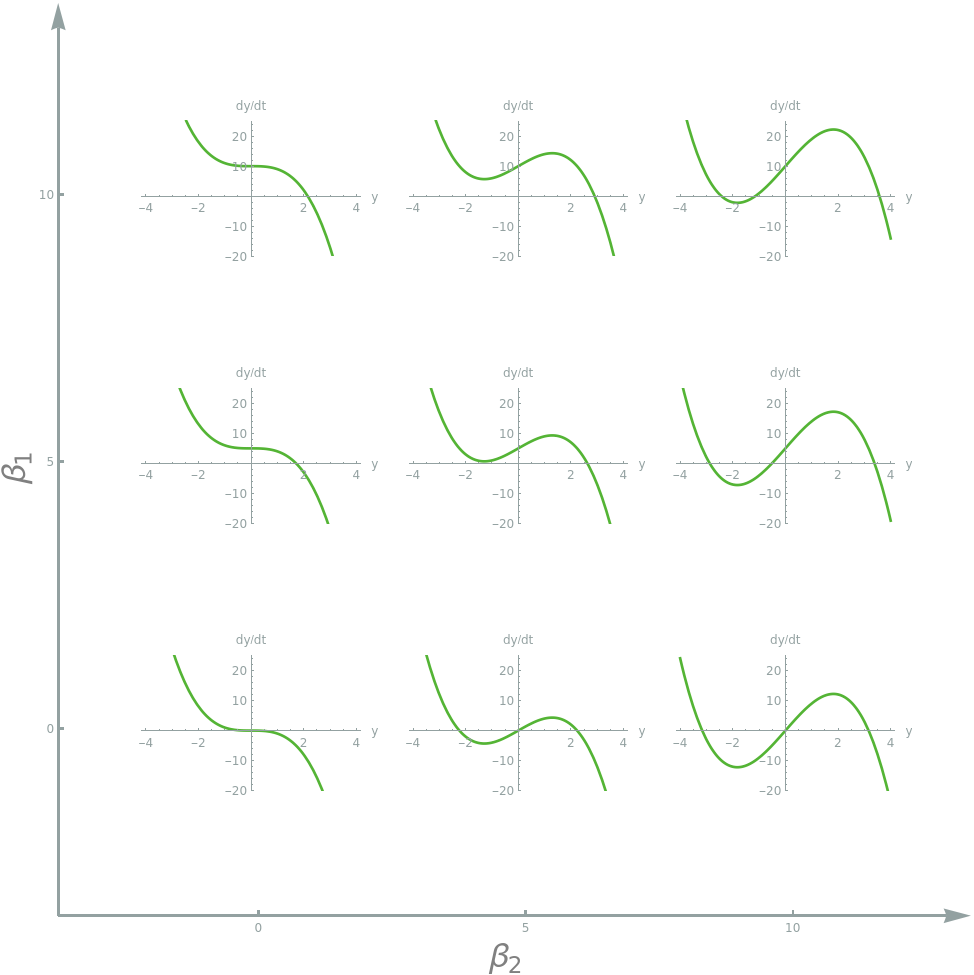
\includegraphics[width=2.1in,angle=0]{./cubic_params.png}
\caption{The effect is that $\beta_2$ determines the curvature around the center
and $\beta_1$ determines where the function reaches equilibrium.
If this is within the curved region this is an example of bistability.}
\label{fig1}
\end{center}
\end{figure}

We are interested in the case where one samples from the state space of
this system at random. We must make an assumption about the form this sampling
procedure takes. We will assume the sampling distribution is a 
uniform distribution within a bounded state range for all three cases. 
Although the method is generic and can
be used for any sampling distribution we will use a uniform distribution 
since it is both the maximum entropy distribution and provides a simple 
way to conceptualize the method.

Since this a one-dimensional bistable system whether a given trajectory ends
in one state or the other is simply a function of whether it is greater than
or smaller than the saddle point position. This is thus equivalent to asking for the
cumulative distribution function of the sampling distribution $CDF(x<X)$ where
$X$ is the position of the unstable equilibrium point (Figure \ref{fig2}).

\begin{figure}[t]
\begin{center}
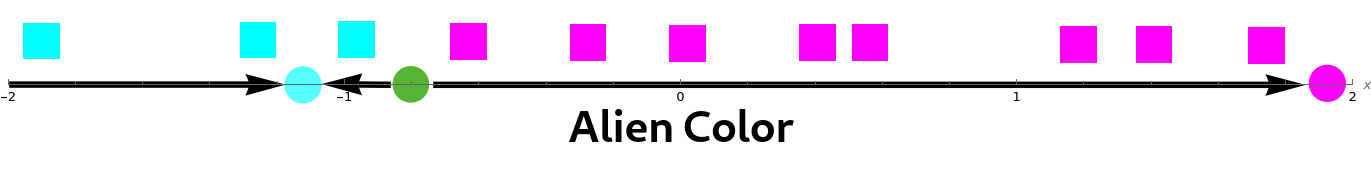
\includegraphics[width=2.1in,angle=0]{./basins.png}
\caption{Here we see the phase portrait of the system. The blue points represent
the stable equillibria and the red points is the saddle node. The magenta volume
represents the region of points that will end up in one basin and the cyan volume
represents the rest of the volume which will end up in the other basin of attraction.}

\label{fig2}
\end{center}
\end{figure}

The CDF relates the position of the unstable equilibrium point to the 
binomial probability of falling in one basin or another. In the case of the
uniform distribution we write out the cdf:
\begin{eqnarray} 
  CDF(x<X) = \frac{\text{ub} - X}{\text{ub}-\text{lb}}
\end{eqnarray}
Intuitively this is simply the area of the cyan volume in Figure 2 divided by the 
area spanned by the whole volume of cyan + magenta. ub, lb are the upper and lower
bounds.\\
Now the position of the saddle point can uniquely define the resulting
probability of the sampled trajectory entering either basin. To relate this
probability back to the model parameters, we must define the relation from
the parameters $\beta_1$ and $\beta_2$ to the position of the unstable
equilibrium point. In the case of the cubic we can do this analytically.
We relate the two as follows:
\begin{eqnarray}
    \beta_1+\beta_2 y = y^3 + \dot{y}\\
    \dot{y} = 0\\
    \ddot{y} > 0
\end{eqnarray}
We visualize this relation as a surface in Figure 3. Notice that the surface only exist
in a portion of the parameter space. This is a result of the fact that the model exhibits
a bifurcation. Only when the curvature caused by $\beta_2$ is sufficient and the $beta_1$
parameter defines the x-intercept along that curvature is a saddle point defined. It
This also means that the probability of being in the basin is 0 (or 1 depending on
which basin we choose as the basis) for all parameters outside a given range.\\
We can plot the probability as a function of the parameters $\beta_1$ and $beta_2$.
If we only plot the surface where the probability is not $0$ (or $1$) we get the 
familiar looking cusp bifurcation, however in this case the surface is embedded in probability
space and thus has a curvature as a result of the shifting basin sizes.
By specifying a given probability we can 
specify a position for the unstable equilibrium. If we plot the position
of the equilibrium points as a function of the parameters $\beta_1$ and $\beta_2$,
we get the familiar looking cusp bifurcation. We can embed that cusp bifurcation
in a 3D space by adding the probability distribution defined by a given point in 
parameter space as the third dimension (Figure \ref{fig4}).

\begin{figure}[t]
\begin{center}
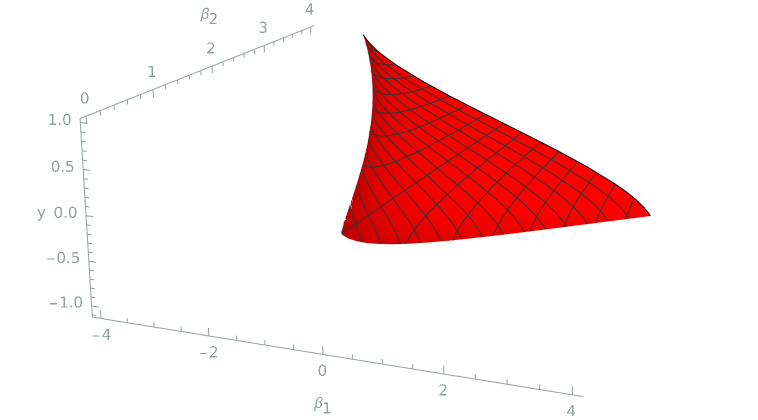
\includegraphics[width=2.1in,angle=0]{./saddle_cubic.png}
\caption{This is the surface of the saddle point location as a function of
the parameter $\beta_1 and \beta_2$.}
\label{fig3}
\end{center}
\end{figure}

\begin{figure}[t]
\begin{center}
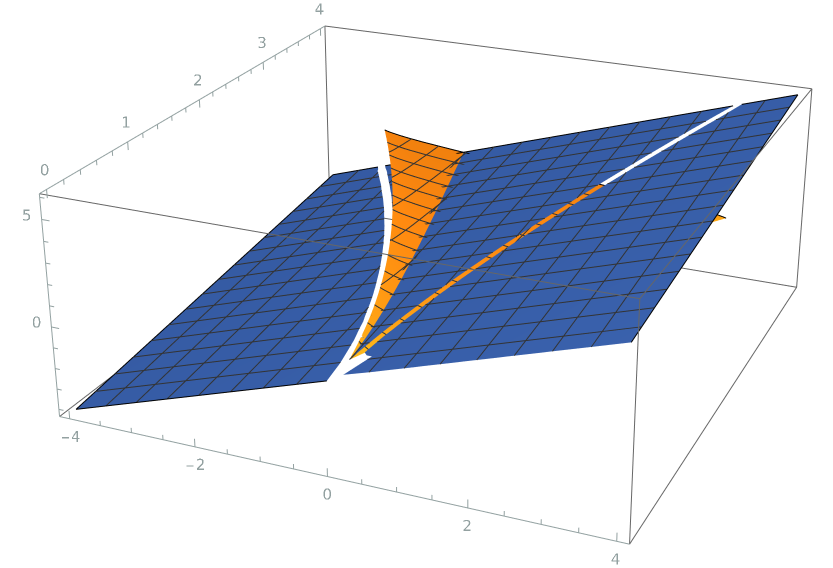
\includegraphics[width=2.1in,angle=0]{./cubic_pg.png}
\caption{This is the surface of the saddle point location as a function of
the parameter $\beta_1$ and $\beta_2$.}
\label{fig4}
\end{center}
\end{figure}

Given that visualization we can simply draw a plane at the desired probability point
in the z-axis. For the purposes of visualization we will assume our desired probability
is $0.7$.
This defines a line or a relation between $\beta_1$ and $\beta_2$ that must be
preserved for the system to have the given probability that it does. Which in this case
can be explitly be written as 
\begin{eqnarray} 
  c = 0.343 - 0.7d
\end{eqnarray}

\subsection{Infant Prehension}
In the previous section we demonstrated how this method can be applied to a simple
toy model and how given an experimentally observed probability we could make a prediction
about the model parameters. However, in many cases the exact model parameters are 
not singular observables but instead are a function of observables. In such cases we 
must accommodate the method by relating the saddle point position not to the model
parameters but to the desired experimental observable.\\
This will be the case as we apply the method to a model of the development of 
reach-to-grasp in infants. Experiments reveal what seems to be a phase transition 
during infant development of prehension. \\
In this case it is observed that infants go 
from reaching to an object to reaching and grasping for an object where over an extended
period of time of 8 weeks (cite) the probability of exhibiting one of the two behaviors 
remains constant. This is true across infants even though the observable parameters
that are used for the model seem to vary over this period. The fact that this probability
remains constant thus might imply a fixed relation between parameters such as the line
we observe in the case of the cubic.\\
We will consider this dynamical model of prehension bistability:
\begin{eqnarray}
  \beta_1 + \beta_2 (\frac{x-51.04}{26.98}) - (\frac{x-51.04}{26.98})^3
\end{eqnarray}
where
\begin{eqnarray}
  \beta_1 = 5.98 - 1.07f + 31.92g\\
  \beta_2 = 5.56 - 0.25f + 0.38g
\end{eqnarray}
Notice that this equation is quite similar to the cubic however both $\beta_1$ and 
$\beta_2$ are linear sums of other parameters: $f,g$ where $f$ is the arm circumference
of the infant and $g$ is the arm weight. In this case, we relate the saddle point 
location to these parameters instead of the cubic paramaters(Figure \ref{fig5}).

\begin{figure}[t]
\begin{center}
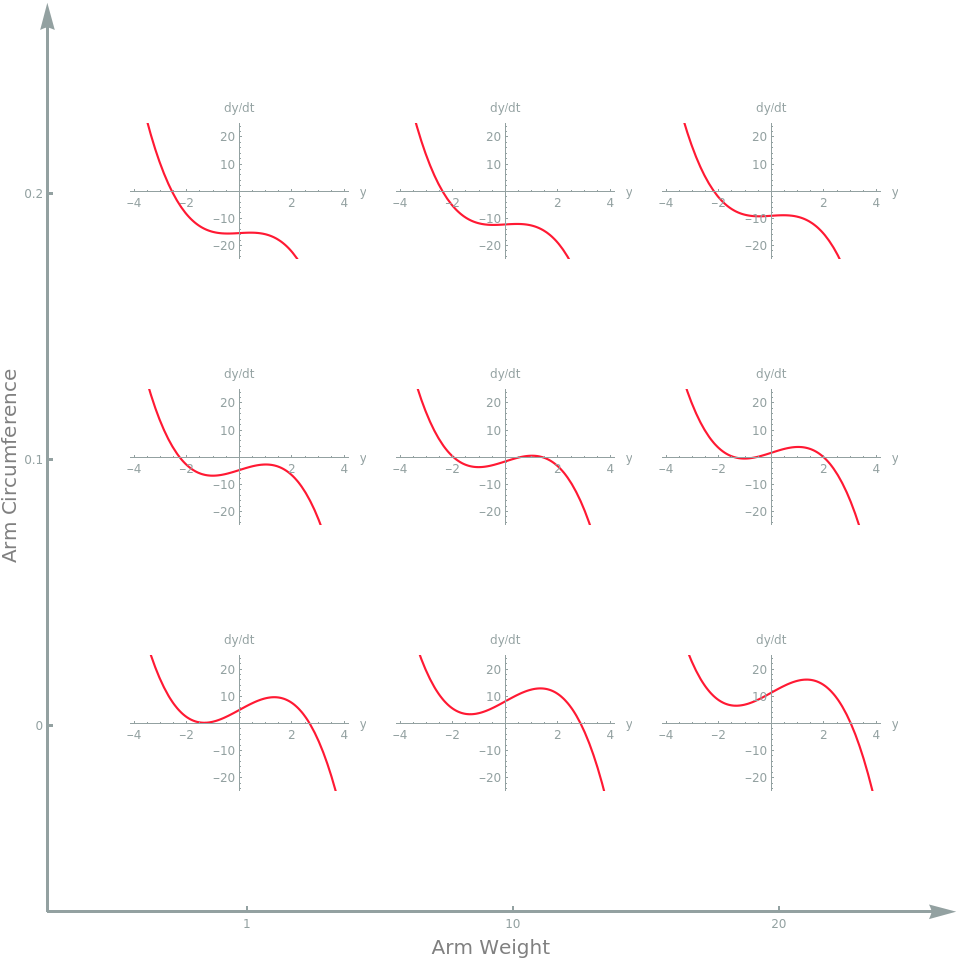
\includegraphics[width=2.1in,angle=0]{./prehension_params.png}
\caption{3x3 grid of variation in $f,g$ and resulting manifold}
\label{fig5}
\end{center}
\end{figure}

In this case since the parameters are linear functions of the observables we can
still simply solve for the saddle point location analytically giving us the saddle 
point as a function of the observables,visualized in Figure \ref{fig6}. 

\begin{figure}[t]
\begin{center}
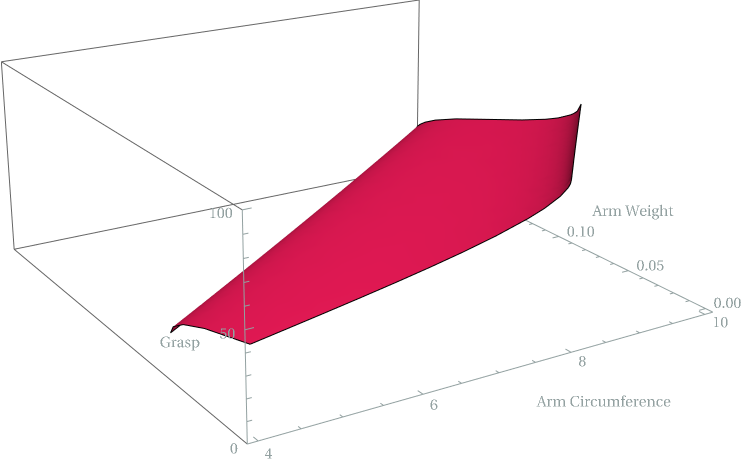
\includegraphics[width=2.1in,angle=0]{./saddle_prehension.png}
\caption{The position of the saddle point as a manifold in parameter space as we vary
parameter $f,g$.}
\label{fig6}
\end{center}
\end{figure}

We can again draw the bifurcation diagram in the 
3D space and intersect it with the probability plane. Once again using the uniform CDF
and taking the inverse function to find the saddle points that satisfy 
our binomial probability distribution of 0.5 we are able to solve for where the 
bifurcation plane and the probability plane intersect

Once again we get a line that relates the two observables $f,g$ with the equation:
\begin{eqnarray}
  \text{prehension line}
\end{eqnarray}
We may make a prediction that the fixed probability distribution implies that the
relation between arm circumference and arm weight follow the equation above during
the 8 week period of constant probability.

\subsection{Planerian Regeneration}
Finally, we consider the case where the bistable equation is not a cubic. Instead
here we look at the regenetation of the planarian flatworm. In the case of plenaria,
experimental observation has found that head-tail patterning utillizes bioelectrical
signaling between cells. Changes in bioelectrical environment of the organism can
lead to a planerian flatworm that develops two heads instead of one. However, it is 
also possible for worms to generate descendant cryptic worms. Such cryptic 
worms after being cut may develop into normal worms or two-headed worms with a
fixed probability. \\
\begin{eqnarray}
  \text{worm model equations}
\end{eqnarray}
Cryptic worms have been interepreted as maintaing a bistable
dynamic where they may fall into the attractor basin of one or two-heads after being
cut. This dynamic has been explored in a simplified model which was able to make 
some predictions that reinforce the idea this system is bistable. However, the model
also shows that basin sizes change as a function of parameter variation which is 
inconsistent with the observation that cryptic worms universally express a probability
of 0.3 in growing two heads (cite).\\
The method we propose can help us better understand this discrepency by directing 
us to consider how the relevant parameters of the model must be related for such a 
fixed probability distribution to emerge.\\
We will use the same methodology as before although in this case we cannot simply
determine the saddle point location as a function of the parameters analytically.
Rather we must use a numerical method to relate the saddle point location to the
parameters of the model (Figure \ref{fig7}).
\begin{figure}[t]
\begin{center}
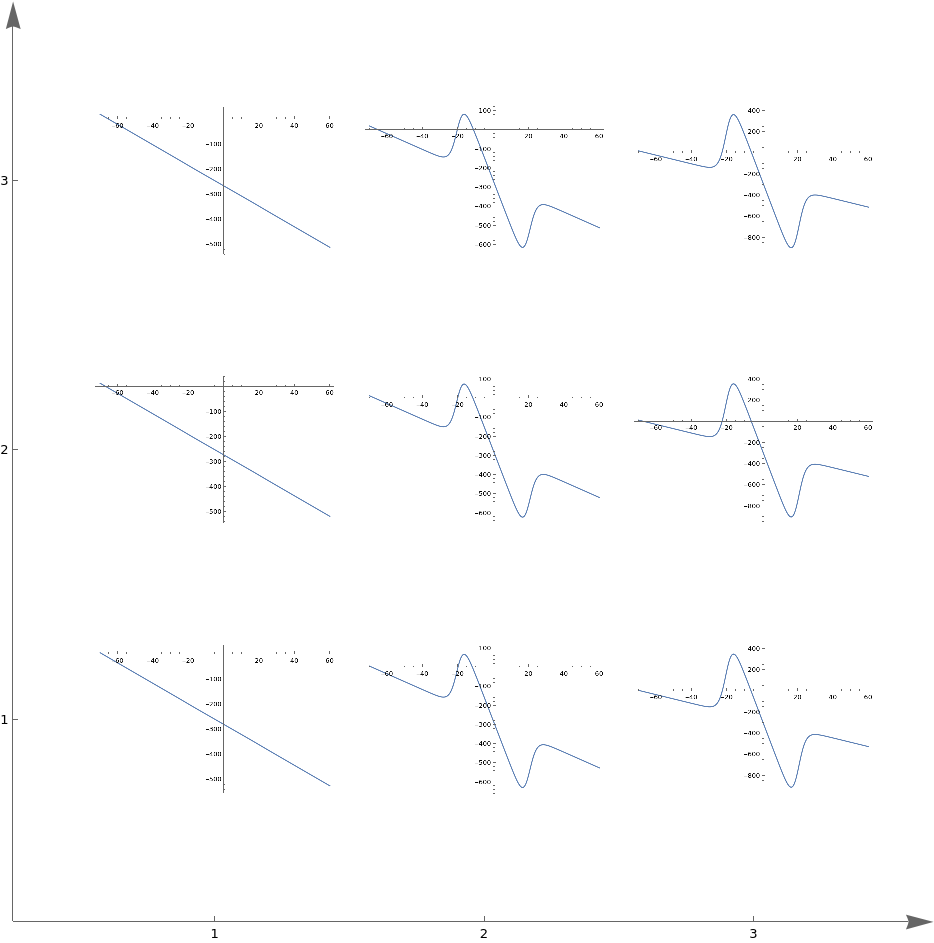
\includegraphics[width=2.1in,angle=0]{./worm_params.png}
\caption{Saddle point location as a function of the two parameters}
\label{fig7}
\end{center}
\end{figure}

Again, we can identify the appropriate 
position of the saddle point based on the known binomial probability of 0.3. This 
allows us to plot the bifurcation diagram across the probability axis as before and find
the intersection of the bifurcation with the plane at $p=0.3$.

\begin{figure}[t]
\begin{center}
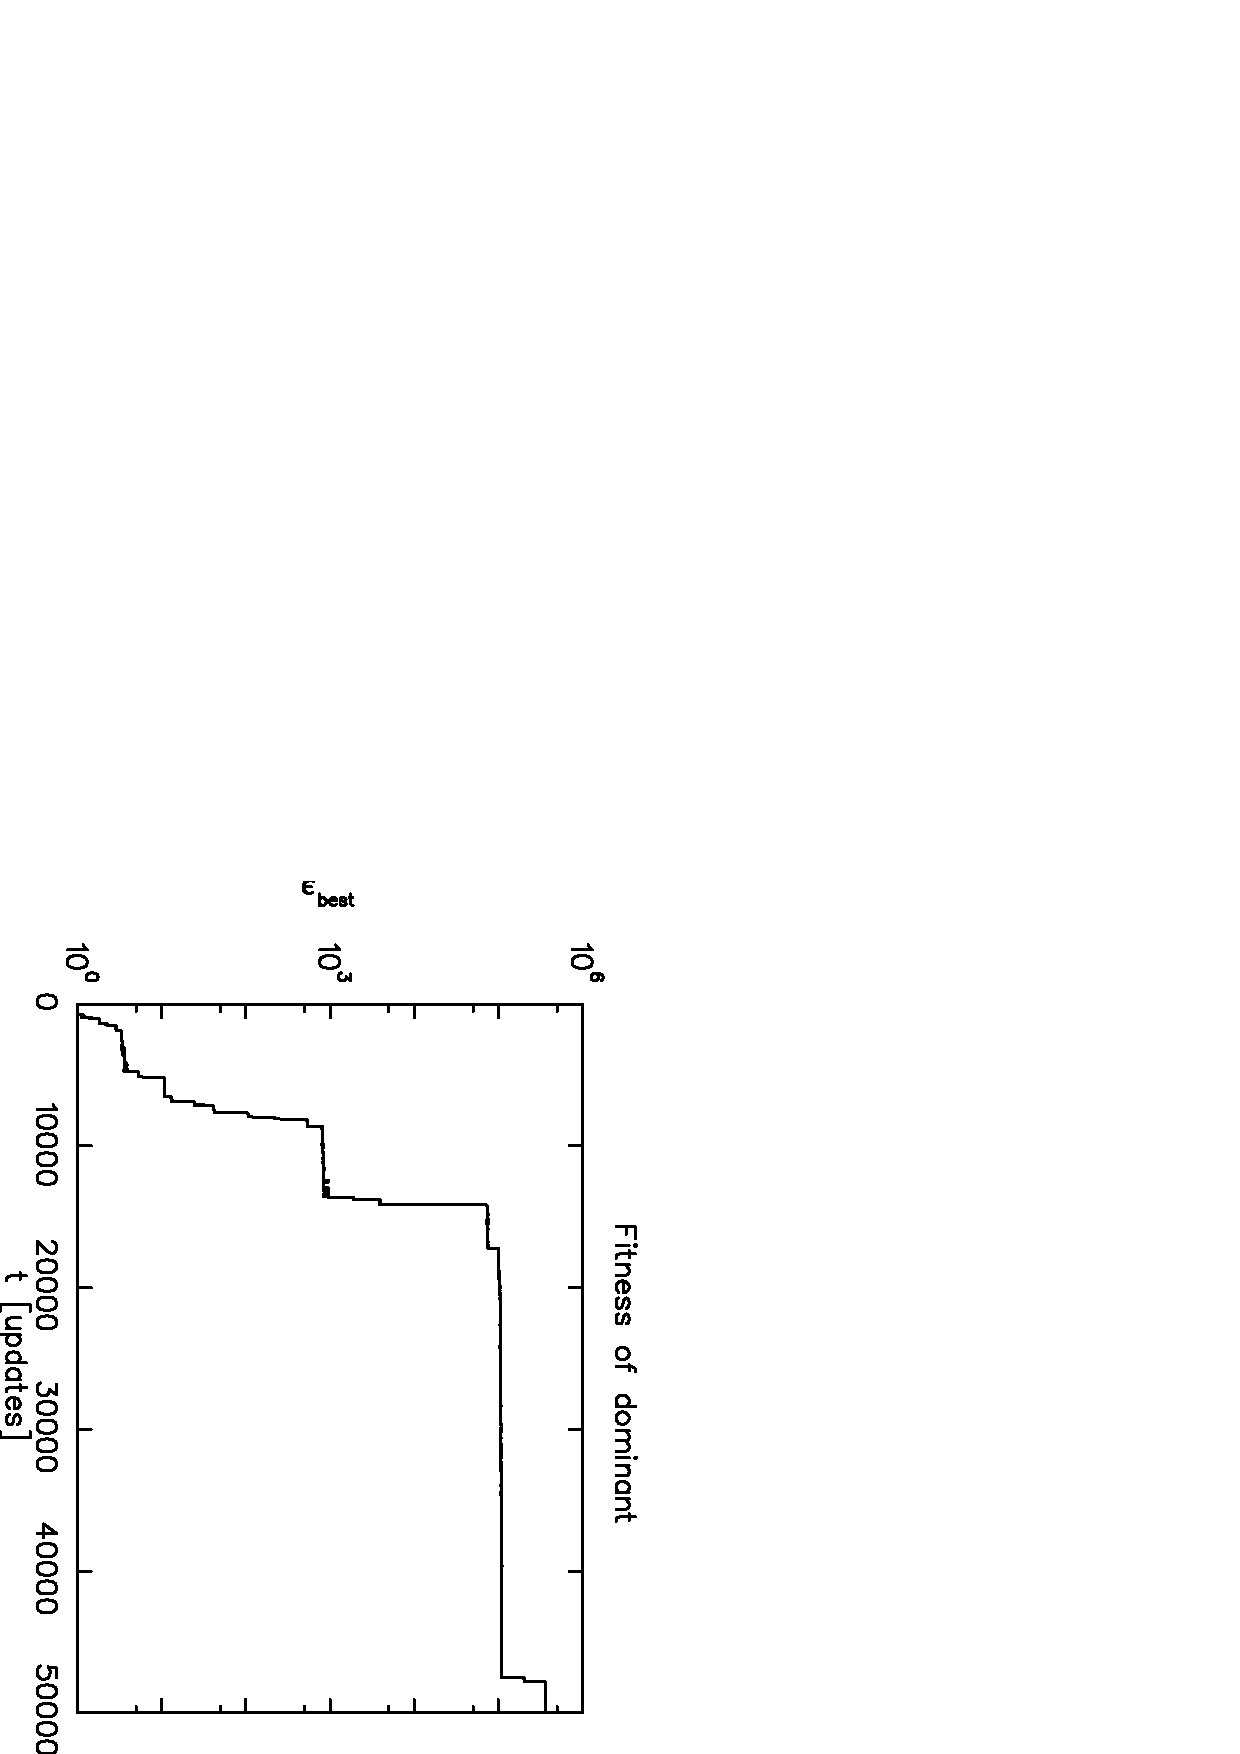
\includegraphics[width=2.1in,angle=-90]{./fig2.png}
\caption{Bifurcation in probability space}
\label{fig6}
\end{center}
\end{figure}

Unlike before we cannot define this intersection analytically however we can
generate a table of values that predicts how the two parameters must be related
if the probability remains constant. We can then plot table to see the relationship
more clearly.

\begin{figure}[t]
\begin{center}
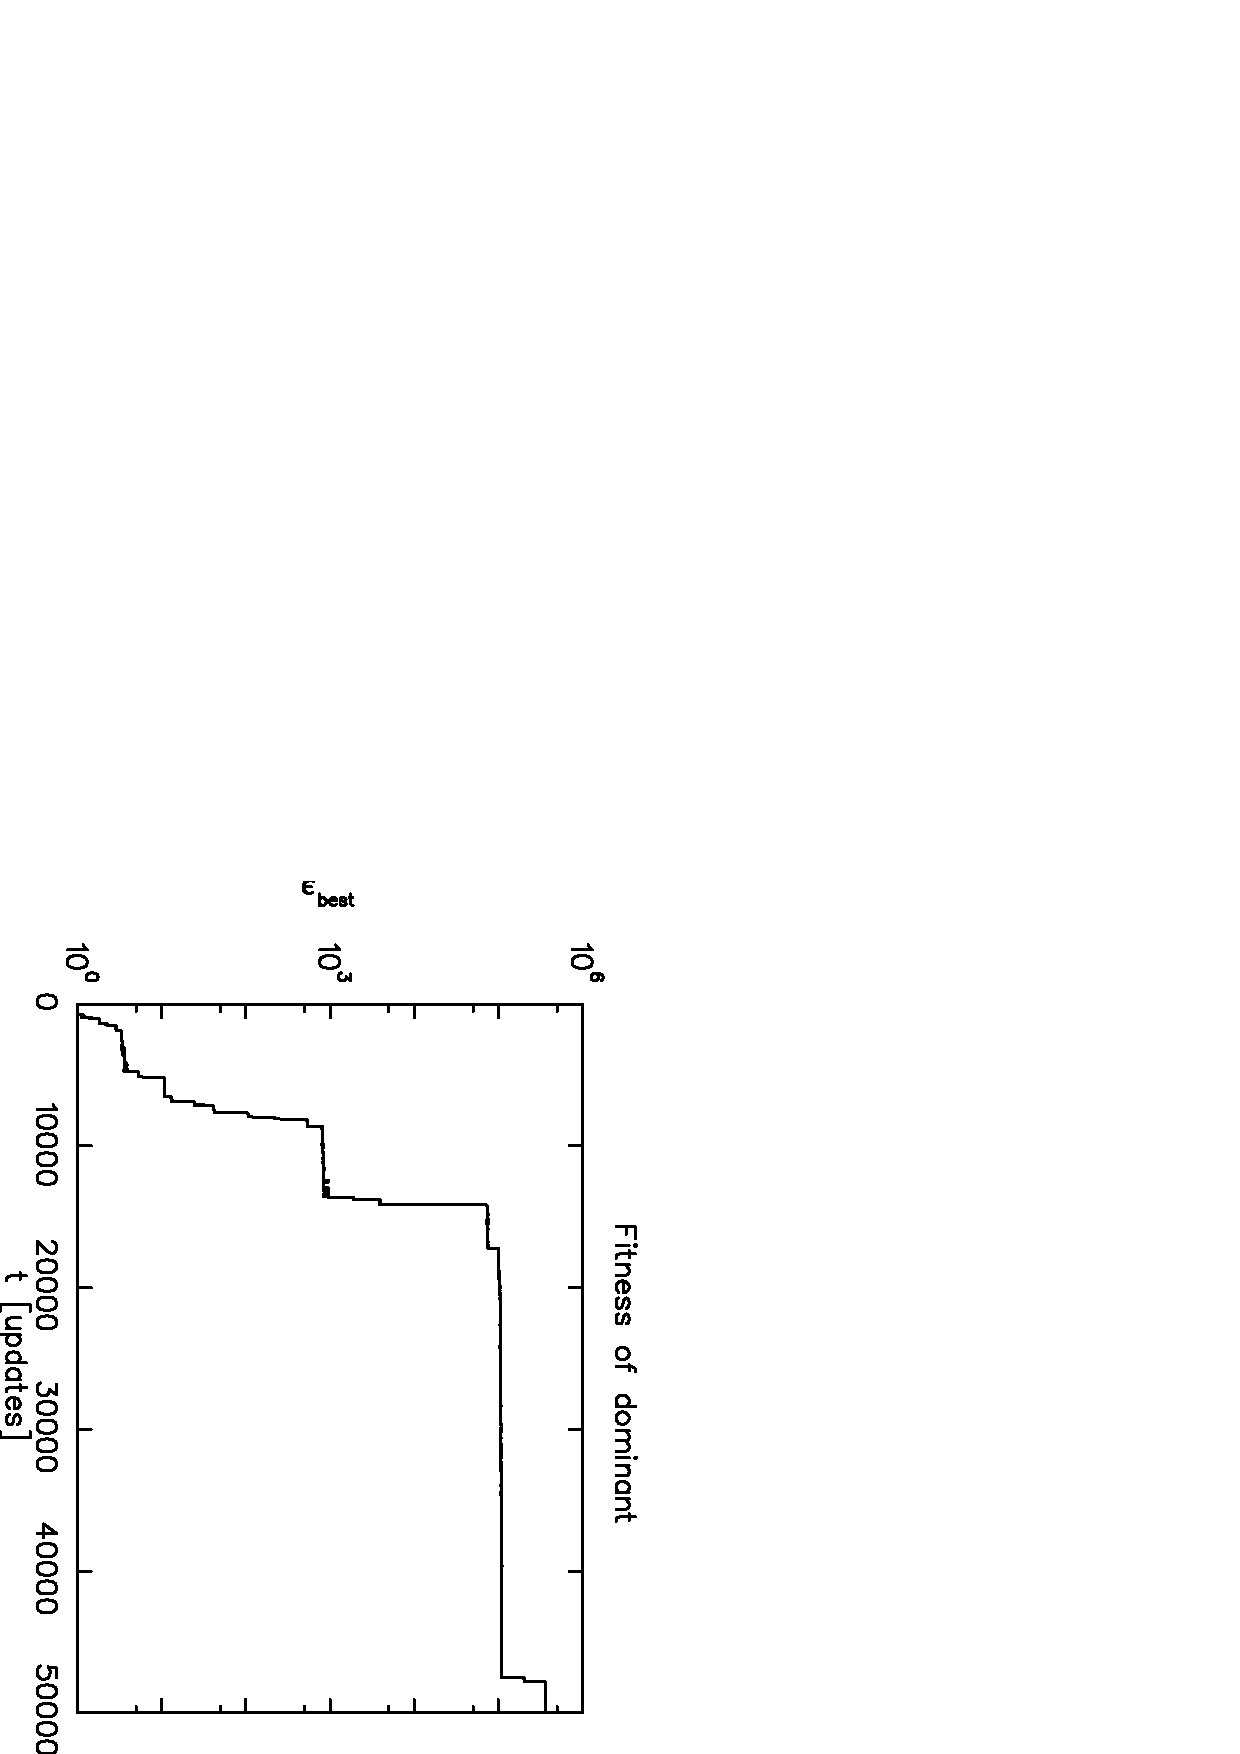
\includegraphics[width=2.1in,angle=-90]{./fig2.png}
\caption{Worm parameters plot}
\label{fig7}
\end{center}
\end{figure}

From here we can see how the constant probability distribution presents a set of 
constraints on the parameters of the dynamical model. In turn such constraints can
be used to make emprical predictions which can further validate or contradict the
model as a hypothesis.

\section{Discussion}

\pagebreak

\section{Acknowledgements}

This work was supported by NSF grant No.\ PHY-9723972.

\footnotesize
\bibliographystyle{apalike}
\bibliography{example} % replace by the name of your .bib file


\end{document}
